\documentclass[11pt, a4paper]{report}
\usepackage[utf8]{inputenc}
\usepackage{float}
\usepackage{array}
\usepackage{amsmath}
\usepackage{amssymb}
\usepackage{amsfonts}
\usepackage{latexsym}
\usepackage{graphicx}
\usepackage{tabularx}
\usepackage{ltxtable}
\usepackage{longtable}
\usepackage{color, colortbl}
\usepackage{caption}%\usepackage{subcaption}
\usepackage{ifpdf}
\usepackage[hidelinks]{hyperref}
\usepackage{url}
\usepackage{xtab}
\usepackage[hmargin=3cm,vmargin=3cm]{geometry}
\usepackage[norsk]{babel}
\usepackage[parfill]{parskip}
\usepackage{pdfpages}
\usepackage{listings}
\usepackage{subfigure}
\usepackage{xcolor,colortbl}

% Begin chapter numbering
\usepackage[T1]{fontenc}
\usepackage{titlesec, blindtext, color}

\definecolor{gray75}{gray}{0.75}
\newcommand{\hsp}{\hspace{20pt}}
\titleformat{\chapter}[hang]{\Huge\bfseries}{\thechapter\hsp\textcolor{gray75}{|}\hsp}{0pt}{\Huge\bfseries}
% End chapter numbering

% Add numbering to subsubsection
\setcounter{secnumdepth}{3}
\setcounter{tocdepth}{3}

\definecolor{Gray}{gray}{0.9}

% Header packages
\usepackage{fancyhdr}
\pagestyle{fancy}
\rhead{Chapter: \thechapter}

% Custom 
%\newcommand{\newCommandName}{text to insert} % Defines a variable in LaTeX
\newcommand{\comment}[1]{} \comment{This is a block comment wrapped in curly brackets}
%\renewcommand{\thefootnote}{\roman{footnote}}

\begin{document}
%\pagecolor{yellow!30} % Uncomment for debugging floats
\pagenumbering{gobble}


\begin{titlepage}
\begin{center}
\vspace*{1in}
{\LARGE Eksperter i Team}
\par
\vspace{1cm}


\begin{figure}[ht!]
\centering
%
\includegraphics[width=25mm]{images/logo.png}
%\caption{A simple caption}
\label{overflow}
\end{figure}


{\LARGE Stereo}
\par
\vspace{0.6in}
{\LARGE Project report}
\par
\vspace{0.2in}
{\Large Group 1}
\par
\vfill
\par
\vspace{0.5in}
Our names\\ \ldots here\\
\par
\vspace{0.4cm}
\today
\end{center}
\end{titlepage}

%\newpage
%
%\input{section/abstract}

\tableofcontents
\newpage
\pagenumbering{arabic}

%%%
% Put new includes here
%%%

\chapter{Introduksjon}
\section{Gruppen} 
\subsection{Emil Bjørlykhaug}
Går undervannsteknologi, 2-årig master. Har tidligere gått Automasjon ved Hials.
Som folk flest hadde jeg hørt en del snakk om EiT på forehand, noe positivt, noe negativt. 
Jeg hadde ikke noen store forventninger ang. selve prosjektet vi skulle gjennomføre,
 men hadde en del forventninger til det å jobbe i gruppe, og å lære hvordan gruppedynamikk 
fungerer sett fra både et teoretisk og praktisk perspektiv. Jeg har tidligere selv jobbet 
en del i grupper, men oftest har medlemmene av desse gruppene vært folk jeg har kjent 
fra før. I et tilfelle når jeg studerte på Hials hadde foreleser ansvaret med å dele opp gruppe, 
så jeg havnet på en gruppe med bare ukjente personer. Jeg følte dette er en god måte å 
utfordre folk sosialt, og følte jeg i løpet av semesteret ble utrolig godt kjent med de jeg 
måtte jobbe sammen med.
Jeg er ikke av typen som roper høgest i diskusjoner, og kan ofte bli litt passiv i 
gruppesammenhenger om jeg ikke føler jeg har noe å stille med, men håper 
EiT kan gjøre meg til et bedre gruppemedlem. Jeg er positivt innstilt til faget 
og håper på høgt læringsutbytte.

\subsection{David Hovind} Jeg har ikke hørt så mye om EiT fra før så jeg vet ikke helt hva det går ut på. 
Jeg har derfor et åpent sinn til faget og ser på det som en positiv utfordring. 
Som regel så foretrekker jeg ikke gruppearbeid fordi man blir avhengig av alle andre i gruppen og de blir avhengige av deg. 
Av den grunn så liker jeg best å jobbe selvstendig, siden det finnes mange forskjellige typer mennesker og man vet aldri 
hvilke typer mennesker man havner på gruppe med. Jeg forventer å bli bedre til å kjenne meg selv og få litt innsikt i 
hvordan det er å reflektere over gruppearbeidet.

\subsection{Kristoffer Løvall}
Jeg fikk høre litt forskjellig om Eksperter i Team før dette semesteret, men har 
prøvd å holde de negative holdningene til faget ute. Jeg starter semesteret 
derfor semesteret med en positiv innstilling, spesielt siden landsbyens tema 
virker veldig interessant og spennende. Jeg forventer at det blir lærerikt å 
jobbe på tvers av fagfelt og interesser, og at tverrfagligheten bidrar til å 
designe et godt produkt. På grunn av tidligere gruppearbeid i forhåndsbestemte 
grupper med ukjente personer har jeg ikke store forventninger til det sosiale, 
noe som på sitt vis kan være positivt ettersom det da ikke er mye som skal til 
for at dette går over forventning. Jeg har også jobbet relativt mye i grupper 
gjennom porsjekter både på NTNU og Høgskolen i Bergen, der jeg ofte har endt opp 
med å ta ansvar og fungere som en gruppeleder. Jeg vet også at jeg kan bli noe 
kontrollerede når jeg blir veldig engasjert og brenner for noe.  Målet mitt for 
Eksperter i Team er å "prøve noe nytt" og være litt mer tilbakeholden på denne 
fronten, prøve å jobbe på linje med alle andre uten å "ta over" for noen og 
kontrollere alle detaljer. Jeg vil bli enklere å jobbe i team med og lære meg 
selv å godta andres løsninger og akseptere disse som de beste løsningene, selv om 
min opprinnelige tanke var noe helt annet. Når det gjelder det faglige håper jeg 
alle har høye forventninger både når det gjelder engasjement for å ende opp med 
gode løsninger, samt det å få en god karakter i faget.

Dette kapitlet beskriver produktidéens gjennomførbarhet gjennom analyse av 
dens markedsverdi. Her veies produksjonskostnad opp mot salgspris og kvantitet.
Resultatene ligger til grunne for markedstilnærmelse, salg og fortjeneste.

\section{Prisestimat}
Tabell \ref{tab:price-HW} viser en oversikt over estimert kostnad for 
hardwaren som utgjør AutoNuts-systemet, og som dermed må integreres i lastebilen. Alle estimater er ekskludert tilleggskostnader som MVA og frakt.
\newline
\begin{table}[H]
\caption{Prisestimat hardwarekomponenter i Norske kroner.}
\label{tab:price-HW}
\begin{tabularx}{\textwidth}{lcc|r}
	{\bf Del} & {\bf Antall} & {\bf Pris pr. enhet} & {\bf Subtotal}\\
	\hline
	Vibrasjonssensor (piezoelektrisk accelerometer) & 6 & 14 & 84\\
	Mikrokontroller & 3 & 10 & 30\\
	Kabler & 3 & 2 & 6\\
	\hline
	\multicolumn{3}{l}{{\bf Total (NOK)}} &\multicolumn{1}{r}{120}\\
	\hline \hline
\end{tabularx}
\end{table}

Som vist i tabellen over, estimeres det 6 vibrasjonssensorer per lastebil. Dette
tilsvarer 2 per aksling, gitt at en lastebil har 3 akslinger. Per aksling 
estimeres også én mikrokontroller, og 3 kabler (to inn, én ut). Dette gir en 
total på 120 kr. per lastebil, og en subtotal på 40 kr. per aksling.

Produksjonskostnaden for teamet vil, i tillegg til innkjøpsestimatet gjort 
ovenfor, være i dagsverk. Det anslås et minimum på 720 dagsverk fra 
planlegging til produksjon. Kostnadsestimatet per dagsverk er 1200 kr. Dette gir en totalkostnad for systemutviklingen på 864000 kr.

\section{Break even}
Det økonomiske målet med prosjektet er i første omgang å nå ``break even'', 
som vil si å gå i null. Figur \ref{fig:breakeven} viser forholdet mellom 
produksjons- og innstallasjonskostnad og salgsinntekter før produktet når 
vendepunktet fra underskuddsprosjekt til profitt. 
	\newline
	\begin{figure}[H]
		\centering
		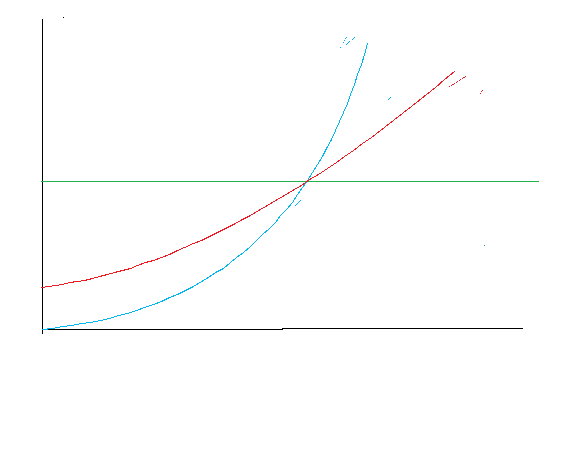
\includegraphics[width=0.80\textwidth]{images/break-even.png}
		\caption{Kostnad vs profitt TODO:fix figur.}
		\label{fig:breakeven}
	\end{figure}
X-aksen viser antall solgte ferdigmonterte enheter, mens Y-aksen viser 
Norske kroner. Rød graf er utgifter, blå graf er inntekter, mens grønn graf 
indikerer prosjektets ``break even'', altså hvor mange enheter som må selges 
før prosjektet går i overskudd.

Kongsberg Automotives representanter anbefalte en salgspris på maksimum 100 kr.
per aksling, noe som gir en total på 300 kr. per bil. Medregnet de beregnede 
dagsverk, må det beregnes et salg på 3324 enheter før prosjektet går i overskudd.

\section{Markedsadgang}
Ettermontering av produktet vil være dyrere enn montering under produksjon av 
lastebil, man må koble fra akslingen for å montere vibrasjonssensor, samt 
trekke kabler og oppdatere software. Ettersom produktet vil bli rimeligst 
dersom det monteres under produksjon av lastebil, vil  samarbeid med en stor 
produsent, slik som feks. Volvo eller Scania være nødvendig for å entre markedet. 

\section{Størrelse på marked}
I de siste fire årene har det blitt produsert over 200 000 lasterbiler årlig 
i Europa \cite{lastebilprod-DAF}. Det vil si at markedet for produktet er 
veldig stort og vi har muligheten til å komme på markedet først. I tillegg er 
det mulighet for gjøre veien tryggere, da færre hjul vil løsne på lastebiler 
som har vårt produkt integrert.

\section{Konkurrenter}
Til nå er det ingen konkurrenter i markedet som har en digital løsning for 
automatisk deteksjon og varsling av løse hjulbolter. Det man kan finne på 
markedet i dage er manuelle løsninger, hvor man fester små indikatorer på 
boltene for å se om de har beveget seg, eller for å feste boltene bedre. De 
eksisterende løsningene kan man lese mer om i kapittel \ref{sec:existing-solutions}.

Vi ønsker å inngå samarbeid med store aktører for å oppnå en nisjerolle i 
markedet. På denne måten ser vi for oss å bli den foretrukne 
underleverandøren av automatisk deteksjon og varsling av løse hjulbolter.

\section{Kundens makt}
Selv om vi har fordelen med å være først ute på markedet med vår løsning vil 
det være flere å konkurrere med om kundene. Da vi er først ut i markedet vil 
vi raskt kunne oppnå en god dialog med kundene. Vi vil etablere oss som en 
fleksibel, løsningsorientert og pålitelig leverandør. Det stilles høye krav 
til komponenter som produseres til lastebiler, da komponentene skal være i 
drift gjennom en lang levetid. Vi vil derfor ha fokus på å levere produkter 
av høy kvalitet til en god pris. Vi skal ha et stort fokus på 
kvalitetssikring for å sikre at ingen produkter med feil havner hos 
sluttbruker. Vi ønsker fornøyde kunder og er derfor mottakelige for nye 
standarder og krav fra kundene. 

\section{Forhold til leverandører}
Det er viktig at vi velger underleverandører som er anerkjent for å levere 
komponenter med høy kvalitet og pålitelighet. Samtidig må vi forholde oss til 
pris på komponenter fra underleverandører, da det vil være vanskelig å få 
solgt produktet til kunder om prisen er for høy. Vi skal kjøpe 
prøveeksemplarer fra forskjellige leverandører for å kunne sammenligne pris 
mot kvalitet. Vi skal sikre gode avtaler med underleverandørene, og binder en 
mindre del av vår kapital på lagerhold om vi har underleverandører som 
leverer komponenter på kort varsel. Vi forhandler frem langsiktige kontrakter 
for å sikre leveranse og pris, med forbehold om brudd ved mislighold av krav 
på kvalitet, pris og levering. 

\section{De fire P-ene}
\begin{description}
	\item[Produktstrategi] De to første årene ønsker vi å starte med utvikling av et enkelt produkt for 		automatisk deteksjon av løse hjulbolter. I år to og tre skal vi jobbe med videreutvikling av 				produktet. Det vil da være aktuelt å se på andre problemer som kan detekteres ved bruk av 			samme sensor. Med tid vil vi da kunne tilby et større produkt, og kunden vil kunne få mer 			funksjonalitet for pengene. Denne videreutviklingen vil fortsette etter de tre årene, helt til all aktuell 		funksjonalitet er implementert.
	\item[Prisstrategi] Delene som kreves for å lage produktet koster ca. 40 kr per aksling for å gjør integrering av produktet mulig. Ettersom vi ikke har innsikt i Kongsberg Automotive sin økonomi, vil prising av produktet være opp til salgsavdelingen deres. Etter hvert som bedriften skaffer seg egenkapital vil det være naturlig å gjøre enda større avtaler med underleverandører og kunder. Dette vil resultere i lavere kostnader ved innkjøp av komponenter og høyere fortjeneste ved salg.
	\item[Distribusjon og salgsstrategi] Vi planlegger å selge produktet til produsenter av lastebiler. De 		skal selge produktet til sine kunder som et tilleggsprodukt eller innbakt i prisen på lastebilen. 			Distribusjon vil derfor gå gjennom produsenter, og fokuset vårt vil være å inngå avtaler med 			produsenter. Vi skal ha et verdensomspennende marked og må derfor inngå avtaler med store 		produsenter slik som Daimler \cite{daimler}. Daimler er verdens største globale produsent av 				trailere over 6 tonn og produsererfor merkene Mercedez, Freightliner, Western Star, Fuso og 			BharatBenz.
	\item[Promoteringsstrategi] Vi skal ha stand på konferanser og messer hvor vi vil vise hvordan vårt 	produkt kan automatisk detetektere og varsle om løse hjulbolter. Her vil vi få kontakt med 			lastebilprodusenter og vise at vårt produkt vil tjene deres produkt. Promotering av produktet vil 		inngå i kundens promotering ut til sluttbruker, da produktet vil være en del av kundens produkt. 		Både kunder og 	sluttbruker vil ha tilgang til informasjon om våre produkter gjennom vår nettside.
\end{description}


\comment{ foreløpig struktur på rapport:
prestudy
	hw
	sw
	markedsundersøkelse
	existing solutions
	hvorfor vår(e) ide(er) er bedre.
designchoises / arkitekturvalg
use cases/arkitektur scetches
tests?
oppsummering
}


%%%
% End includes
%%%

%\newpage
%\addcontentsline{toc}{chapter}{List of Tables}
%\listoftables
%\addcontentsline{toc}{chapter}{List of Figures}
%\listoffigures
%\addcontentsline{toc}{chapter}{Bibliography}
%\bibliographystyle{plain}
%\input{section/bibliography}

%\newpage
%\addcontentsline{toc}{chapter}{Appendixes} % This line may break your compilation, and may require recompiation. Not to worry though.
%\appendix
%\input{section/appendix-someAppendix}


\end{document}
